\documentclass[12pt, oneside]{article}
\usepackage{geometry}
\geometry{letterpaper}
\usepackage{graphicx}
\graphicspath{{images/}}
\usepackage{amsmath}
\usepackage{amsthm}
\usepackage{amssymb}
\usepackage{diagbox}
\usepackage{mathtools}
\usepackage{hyperref}
\usepackage{enumerate}
\usepackage{booktabs}
\usepackage[shortlabels]{enumitem}
\usepackage{tikz}
\usetikzlibrary {shapes.geometric}
\usetikzlibrary{angles,quotes}
\hypersetup{
	colorlinks=true,
	urlcolor=blue
}

\title{Math Journal}
\author{Andrew Ha}
\date{}								%no date

\newtheorem{proposition}{Proposition}
\newtheorem{identity}{Identity}

\begin{document}
\maketitle
\section*{Combinatorial Proof}
\textbf{09/10/2024}
\begin{proposition} For positive integers $n$ and $k$ with $n=2k, \frac{n!}{2!^k}$ is an integer. \end{proposition}
\emph{Proof.}  Consider the $n$ symbols: $x_1, x_1, x_2, x_2, \cdots, x_k, x_k$.
The number of arrangements of all these $n = 2k$ symbols is an integer that equals
\[
\frac{n!}{\underbrace{2! 2! \cdots 2!}_{\text{k factors of 2!}}} = \frac{n!}{2!^k}
\]
I learned this from the first day of class in MACM 101. This is an example of proving that a value is an integer by obtaining that value from counting something. Researching further, I also found out about double counting.\ It is based on the idea that counting the same objects in two different ways results in two different expressions, which must be equal to each other. 
\begin{identity}
\[
2^n = \sum_{k=0}^{n}  \binom{n}{k}
\]
\end{identity}
For example, this identity can be proved by counting the number of subsets of a set $A$ with $n$ elements. One way to count this is noticing how you can either include or exclude each element, giving 2 choices for each of the $n$ elements. This gives $2^n$ subsets. Second way to count the number of subsets is summing up the number of subsets with $k$ elements where $k$ can be any integer from 0 to $n$. For each case, you would be choosing $k$ elements out of $n$ elements, so there are t$\binom{n}{k}$ subsets.
Summing up, the total number of subsets is $\sum_{k=0}^{n}  \binom{n}{k}$.\ Two expressions, $2^n$ and $\sum_{k=0}^{n}  \binom{n}{k}$, must be equal since they represent the same thing.
\section*{Putnam 2002 B1}
\textbf{09/11/2024}
\\
\noindent Here is a fun problem I wanted to share from the 2002 William Lowell Putnam Mathematics Competition.
\begin{quote}
B1. Shanille O'Keal shoots free throws on a basketball court. She hits
the first and misses the second, and thereafter the probability that
she hits the next shot is equal to the proportion of shots she
has hit so far. What is the probability she hits exactly 50 of
her first 100 shots?
\end{quote}
This problem doesn't require much of advanced mathematics, yet it is simple and tricky. Here's a solution I like:\\

\emph{Solution.} The probability of $n$th success is the proportion of shots she has hit so far, which is $\frac{n - 1}{\text{\# of shots so far}}$. On the other hand, the probability of $n$th miss is $1 - \frac{\text{\# of successes so far}}{\text{\# of shots so far}} = \frac{\text{\# of shots so far}}{\text{\# of shots so far}} - \frac{\text{\# of shots so far} - (n - 1)}{\text{\# of shots so far}} = \frac{n-1}{\text{\# of shots so far}}$. For her to hit exactly 50 of her first 100 shots, she has to hit exactly 49 shots and miss exactly 49 shots. Consider the probability of one case where she hits 49 shots consecutively then misses 49 shots consecutively: 
\[
\underbrace{\frac{1}{2} \times \frac{2}{3} \times \frac{3}{4} \times \frac{4}{5} \times \cdots \times \frac{49}{50}}_\text{49 successes} \times \underbrace{\frac{1}{51} \times \frac{2}{52} \times \frac{3}{53} \times \frac{4}{54} \cdots \times \frac{49}{99}}_\text{49 misses} = \frac{49!^2}{99!}
\]
Here, the arrangement of shots does not affect the overall probability since the numerator will always be $49!^2$ as long as she hits 49 shots and misses 49 shots, and the denominator will always be 99!. Therefore, multiplying the probability of single case by the number of arrangements will give us the answer. The number of arrangements of 49 shots and 49 misses is $\frac{98!}{49!^2}$ since there are 49 duplicates of 2 cases. Multiplying two numbers yields
\[
\frac{49!^2}{99!} \cdot \frac{98!}{49!^2} = \frac{1}{99}
\]
The probability she hits exactly 50 of her first 100 shots is $\dfrac{1}{99}$.
\pagebreak
\section*{Two Random Distributions}
\textbf{09/16/2024}
\\
This is from a \href{https://www.youtube.com/watch?v=ga9Qk38FaHM}{YouTube video} I watched recently. It talks about a surprising fact that choosing a random number between 0 and 1 and calculating its square root is actually the same as choosing two random numbers between 0 and 1 and taking the larger one. To see why, we look at the distribution of two functions, max($X, Y$) and $\sqrt{X}$. $X$ and $Y$ are independent and random numbers between 0 and 1. Since two distributions are continuous, the probability of getting a specific number is 0. Instead, we look at the probability of getting a number less than or equal to $n$. For max($X, Y$), both $X$ and $Y$ must be less than or equal to $n$. Notice that the probability of getting a number less than or equal to $n$ is $n$ since it is between 0 and 1.
\[
P(\text{max}(X, Y) \leq n) = P(X \leq n) \cdot P(Y \leq n) = n^2
\]
Now, for $\sqrt{X}$, $X$ has to be less than or equal to $n^2$ for $\sqrt{X}$ to be less than or equal to $n$.
\[
P(\sqrt{X} \leq n) = P(X \leq n^2) = n^2
\]
This can actually be generalized that choosing a max value of $m$ random numbers between 0 and 1 and taking the $m$th root of a random number between 0 and 1 are identical. 
\begin{eqnarray*}
P(\text{max}(X_1, X_2, \cdots, X_m) \leq n) = & P(X_1 \leq n) P(X_2 \leq n) \cdots P(X_m \leq n) & = n^m\\
P(\sqrt[m]{X} \leq n) = & P(X \leq n^m) & = n^m
\end{eqnarray*}
This reminds me of what I learned in statistics about probabilities.
\section*{$\bigwedge$}
\textbf{09/17/2024}\\
I had a funny thought while walking to school today. I imagined two bicycles coming from opposite sides of a road that narrows suddenly in the middle of them. There would be two types of people, people who slow down for the other person to pass first (call them D) and people who speed up to pass faster than the other person (call them U). If D and D meet, or if U and D meet, there will be no accident. However, if U and U meet, there will be an accident. I thought of the truth table for AND ($\wedge$).
\begin{center}
\begin{tabular} {| c | c | c |}
\hline
$p$ & $q$ & $p \wedge q$\\
\hline
T & T & T\\
\hline
T & F & F\\
\hline
F & T & F\\
\hline
F & F & F\\
\hline
\end{tabular}
\end{center}
Asking "accident?", D say no (F), and U say yes (T). Two meeting in the road is the AND operation, so the result comes out as the truth table suggests.
\section*{Intro Puzzle from Jane Street}
\textbf{09/21/2024}\\
Last school year, I got an email from the Mathematical Association of America leading me to the \href{https://www.janestreet.com/puzzles/}{puzzles page} in Jane Street. This is the intro puzzle:
\begin{quote}
\textbf{Why Puzzles}

What’s a company like Jane Street doing with a page about puzzles? The act of solving puzzles, though that might seem abstract, is intrinsic to the work we do at Jane Street.

Only by identifying new problems in the financial markets and figuring out (potentially novel) ways to solve them can Jane Street continue to thrive. Even though we have established strategies, we’re humble enough to know that if we have a good idea, others may soon have it as well. Prime among the skills necessary to stay successful, then, is creative problem solving, or puzzling.

Number puzzles, logic puzzles, puzzles with and without clear answers, puzzles with and without clearly defined rules — these are all part of day-to-day life at Jane Street, which is why we’ve chosen to devote this section of our website to puzzles. Plus, solving puzzles just feels great.

One last thing — this is a puzzle!
\end{quote}
At first, I spent about 30 minutes just staring at the text.\ Eventually I found the way to decode it; I just needed to look at the capitalized words. Bringing out all the capitalized words, it reads "What's The Only Even Prime Number Plus One", so the answer is $2+1=3$.

Jane Street has been positng a puzzle every month since 2014, and some are challenging while some are doable (especially the older ones). I tried the \href{https://www.janestreet.com/puzzles/hooks-index/}{second oldest puzzle} where you need to enter nine 9’s in the outermost hook, eight 8’s in the next hook, then seven 7’s, six 6’s, and so on, down to the one 1 (already entered), so that the row and column sums match the values given along the border.\\
\begin{center}
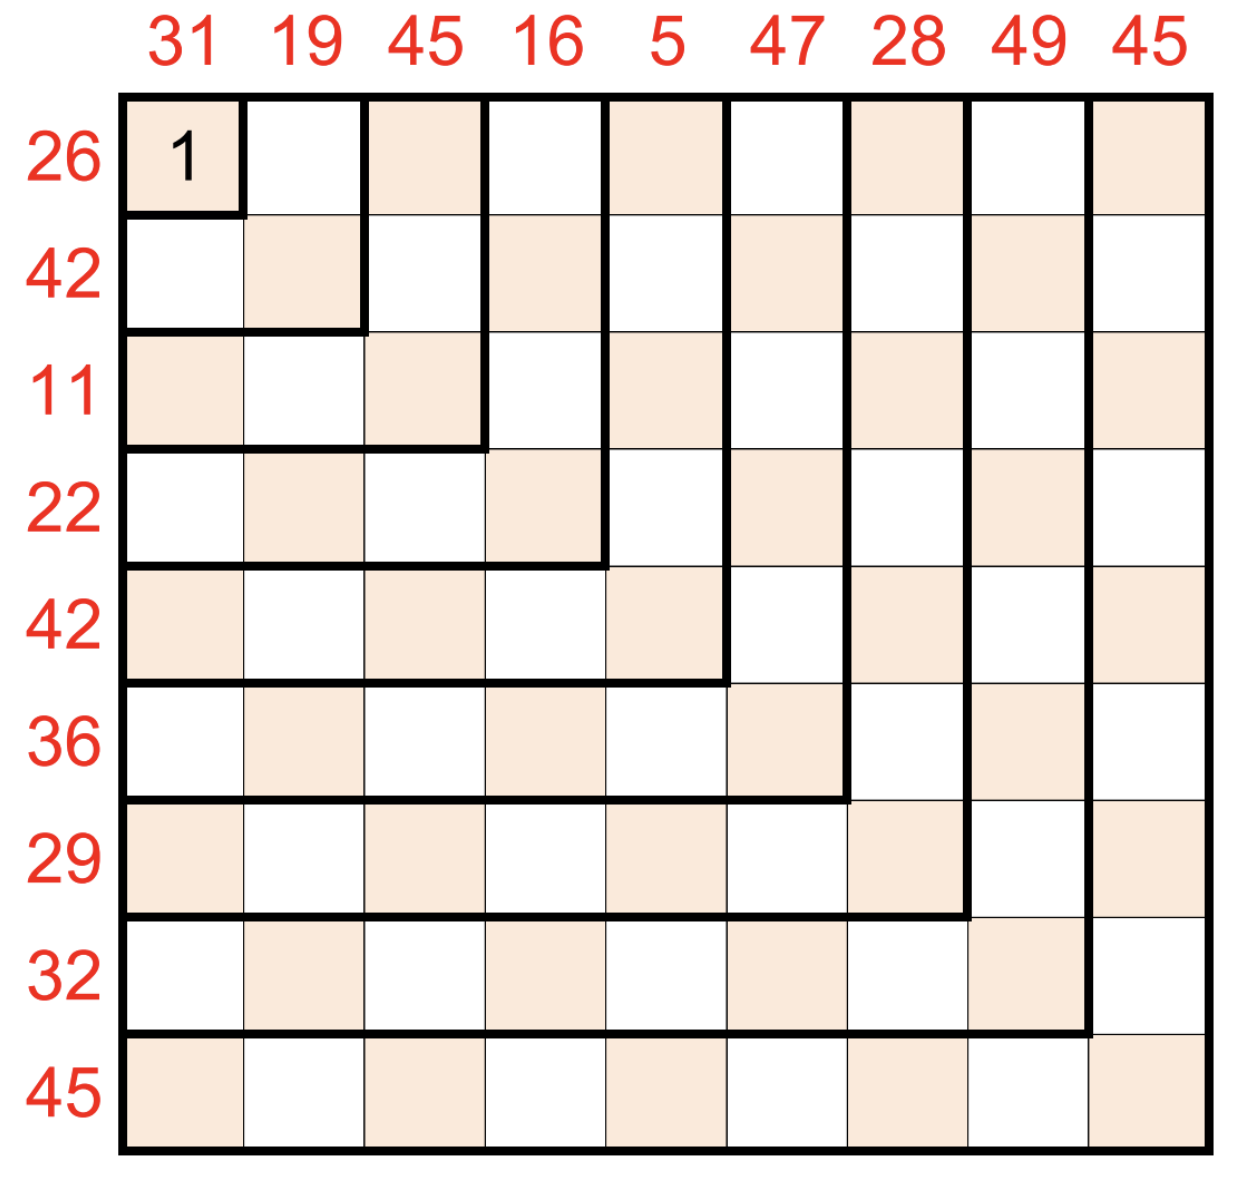
\includegraphics[scale=0.4]{puzzle1}
\end{center}
It was easy to solve given enough time because I could fill out the grid from the bottom right corner one by one. I figured that it would be easy to manipulate the answer (eg.\ add/multiply certain squares) so I can get the number I want with  puzzles similar to this.
\section*{A Counting Problem}
\textbf{09/23/2024}\\
This is a counting problem I struggled to solve without any hints. 
\begin{quote}
For $n \geq 4$, consider the strings made up of $n$ bits --- that is, a total of n 0's and 1's. In particular, consider those strings where there are (exactly) two occurrences of 01. How many such strings are there?
\end{quote}
I wrote down the small cases to find a pattern. 
\begin{center}
\begin{tabular} {|c|c|c|c|c|}
\hline
 \diagbox{$n$}{\# of 01} & \textbf{0} & \textbf{1} & \textbf{2} & \textbf{3}\\
 \hline
 \textbf{4} & 5 & 10 & 1 & 0\\
 \hline
 \textbf{5} & 6 & 20 & 6 & 0\\
 \hline
 \textbf{6} & 7 & 35 & 21 & 1\\
 \hline
 \textbf{7} & 8 & 56 & 56 & 8\\
 \hline
\end{tabular}
\end{center}
I counted the small cases with hand, and I used that the sum of the numbers in a row must add up to $2^n$ to fill the rest of the table. After completing the third row, I noticed that all the numbers in $n$th row are from $(n+1)$th row of Pascal's triangle, so I used this fact to complete the fourth row. I eventually guessed the formula for the number of binary strings of length $n$ with $k$ 01s to be $\binom{n+1}{2k+1}$. However, I could not figure out how choosing $2k+1$ out of $n+1$ objects can represent a binary string of length $n$ with $k$ 01s. I examined the specific case of $n=6$, $k=2$ and $\binom{n+1}{2k+1} = \binom{7}{5}$. I counted how many times 0 switches to 1 or 1 to 0 for the string to have 2 occurrences of 01, and there were 4 cases if I shortened any repeating digits to just one of them. \\

\begin{tabular}{c l l}
1) & 0101 & Switches 3 times\\
2) & 01010 & Switches 4 times\\
3) & 10101 & Switches 4 times\\
4) & 101010 & Switches 5 times\\
\end{tabular}\\

\noindent I realized that you can merge all four cases by putting 1 at the front and 0 at the end.\\

\begin{tabular}{c l c l}
1) & 0101 & $\rightarrow$ & 101010\\
2) & 01010 & $\rightarrow$ & 101010\\
3) & 10101 & $\rightarrow$ & 101010\\
4) & 101010 & $\rightarrow$ & 101010\\
\end{tabular}\\

\noindent With extra 1 and 0, there are now 8 letters and thus 7 places (between each letter) where 0 and 1 can be switched, and they are always switched 5 times. We now choose 5 out of 7 places to have exactly 2 occurrences of 01, so we obtain the desired number, $\binom{7}{5}$. To generalize, there are $\binom{n+1}{2k+1}$ strings with exactly $k$ occurrences of 01 and length $n$. Thus, the answer we are looking for is $\binom{n+1}{5}$.
\section*{Putnam 2013 A1}
\textbf{09/24/2024}\\
Here's another simple problem from the Putnam competition. 
\begin{quote}
Recall that a regular icosahedron is a convex polyhedron having 12 vertices and 20 faces; the faces are congruent equilateral triangles. On each face of a regular
icosahedron is written a nonnegative integer such that
the sum of all 20 integers is 39. Show that there are
two faces that share a vertex and have the same integer
written on them.
\end{quote}
When I tried this problem, I tried to figure out the maximum number of same integer that can be written by drawing out the icosahedron and trying to put in single number as many as possible. I was able to put 4 without a sharing vertex, but I wasn't able to find a way to put 5. I figured 4 was the maximum although I couldn't think of a way to prove it. To minimize the sum, I needed to put 5 smallest nonnegative integers (0, 1, 2, 3, 4) 4 times each which gives the sum of $4 \cdot (0 + 1 + 2 + 3 + 4) = 40$. Thus, the sum of 39 cannot be achieved without two faces sharing a vertex and having the same integer written on them. This solution is valid if I could prove that 4 is the maximum number of same integer that can be written.

It turned out that there was a simple and beautiful proof for it. If the same integer is written on 5 different triangular faces, and none of the vertices are shared, then there are 15 different vertices in an icosahedron. Since there are only 12 vertices in an icosahedron,  the maximum number of same integer that can be written is 4.

Asking what the minimum sum of the numbers with no two faces that share a vertex and have the same integer instead of proof questions will allow this problem to be used in Lockbox. The conditions can also be adjusted to get a number we want.
\section*{Linear Recurrences}
\textbf{09/29/2024}\\
When a term $a_n$ in a sequence $a_1, a_2, a_3, \cdots a_n, a_{n+1}, \cdots$ is defined by its preceding terms, it is a recurrence. It is a linear homogenous reccurrence of degree $k$ if the recurrence relation is in a form \[a_n = c_1a_{n-1} +  c_2a_{n-2} + c_3a_{n-3} + \cdots + c_ka_{n-k}\]  We can obtain an explicit formula for $a_n$ given the relation and the first $k$ terms of the sequence. 

First, we try to find any $a_n = x^n$ with $x \neq 0$ that satisfies the relation. 
\begin{eqnarray*}
x^n & = & c_1x^{n-1} +  c_2x^{n-2} + c_3x^{n-3} + \cdots + c_kx^{n-k}\\
x^{n-k}(x^k & = & c_1x^{k-1} +  c_2x^{k-2} + c_3x^{k-3} + \cdots + c_k)\\
x^k & = & c_1x^{k-1} +  c_2x^{k-2} + c_3x^{k-3} + \cdots + c_k \text{ since } r \neq 0\\
x^k - c_1x^{k-1} +- c_2x^{k-2} - c_3x^{k-3} - \cdots - c_k &=& 0
\end{eqnarray*}
This is called the \emph{characteristic equation}, and we can obtain the roots $x=r_i$ with  $1 \leq i \leq k$ where each $a_n = r_i^n$ satisfies the initial relation. We will first consider the case where all the roots are distinct.

If $r_1^n$ and $r_2^n$ satisfy the relation, $\alpha_1 r_1^n + \alpha_2 r_2^n$ also satisfy the relation. 
\begin{eqnarray*}
r^n & = & c_1r^{n-1} +  c_2r^{n-2} + \cdots + c_kr^{n-k}\\
\Leftrightarrow \alpha r^n & = & c_1\alpha r^{n-1} +  c_2\alpha r^{n-2} + \cdots + c_k\alpha r^{n-k}\\
(\alpha_1 r_1^n + \alpha_2 r_2^n) & = & c_1(\alpha_1 r_1^{n-1} + \alpha_2 r_2^{n-1}) +  c_2(\alpha_1 r_1^{n-2} + \alpha_2 r_2^{n-2}) + \cdots + c_k(\alpha_1 r_1^{n-k} + \alpha_2 r_2^{n-k})\\
\end{eqnarray*}
Therefore, we can combine all the $r_i^n$ to find $a_n$ that not only satisfies the relation but also matches the first $k$ terms.

Here's an example for better understanding. This is a problem from the Canadian Lynx Mathematical Competition 2023.
\begin{quote}
\textbf{\#13:} You are given a biased coin, where Heads comes up with probability $\frac{2}{3}$ and Tails comes up with probability $\frac{1}{3}$.\\\\You play a game where you start with 0 points. Each time you flip Heads, you add 2 points to your score. Each time you flip Tails, you add 1 point to your score.\\\\If you reach \emph{exactly n} points, then you win. However, if you \emph{go over n} points, then you lose.\\\\Let $P_n$ be the probability that you win the game with a target score of $n$ points.\\\\Determine the value of $P_8$.
\end{quote}
First, $P_0 = 1$ and $P_1 = \frac{1}{3}$ trivially. For $n \geq 2$, we can reach exactly $n$ points by flipping Heads with $n-2$ points or flipping Tails with $n-1$ points. This is a linear homogenous recurrence relation:\[P_n = \frac{1}{3}P_{n-1} + \frac{2}{3}P_{n-2}\] With its characteristic equation, I can find two solutions that satisfy the recurrence.
\begin{eqnarray*}
x^2 & = & \frac{1}{3}x + \frac{2}{3}\\
3x^2 & = & x + 2\\
3x^2 - x - 2 & = & 0\\
(3x+2)(x-1) & = & 0\\
x & = & -\frac{2}{3}, 1
\end{eqnarray*}
Since we know $(-\frac{2}{3})^n$ and $1^n$ satisfy the recurrence, we try to find $\alpha_1$ and $\alpha_2$ so $P_n = \alpha_1(-\frac{2}{3})^n + \alpha_2(1)^n$ matches $P_0 = 1$ and $P_1 = \frac{1}{3}$. 
\begin{align*}
&\begin{dcases}
\alpha_1\left(-\frac{2}{3}\right)^0 + \alpha_2(1)^0 & = 1\\
\alpha_1\left(-\frac{2}{3}\right)^1 + \alpha_2(1)^1 & = \frac{1}{3}\\
\end{dcases}\\\\
&\begin{dcases}
\alpha_1 + \alpha_2 & = 1\\
-\frac{2}{3}\alpha_1 + \alpha_2 & = \frac{1}{3}\\
\end{dcases}\\\\
&\begin{dcases}
\alpha_1 & = \frac{2}{5}\\
\alpha_2 & = \frac{3}{5}
\end{dcases}
\end{align*}
We find that $\displaystyle P_n = \frac{2}{5}\left(-\frac{2}{3}\right)^n + \frac{3}{5}(1)^n = \frac{2}{5}\left(-\frac{2}{3}\right)^n + \frac{3}{5}$. We can see that this is valid by substituting:
\begin{eqnarray*}
P_n & = & \frac{1}{3}P_{n-1} + \frac{2}{3}P_{n-2}\\
\frac{2}{5}\left(-\frac{2}{3}\right)^n + \frac{3}{5} & = & \frac{1}{3}[\frac{2}{5}\left(-\frac{2}{3}\right)^{n-1} + \frac{3}{5}] + \frac{2}{3}[\frac{2}{5}\left(-\frac{2}{3}\right)^{n-2} + \frac{3}{5}]\\
& = & \frac{2}{15}\left(-\frac{2}{3}\right)^{n-1} + \frac{1}{5} + \frac{4}{15}\left(-\frac{2}{3}\right)^{n-2} + \frac{2}{5}\\
& = & \frac{2}{15}\left(-\frac{2}{3}\right)^{-1}\left(-\frac{2}{3}\right)^n + \frac{1}{5} + \frac{4}{15}\left(-\frac{2}{3}\right)^{-2}\left(-\frac{2}{3}\right)^n + \frac{2}{5}\\
& = & -\frac{1}{5}\left(-\frac{2}{3}\right)^n + \frac{1}{5} + \frac{3}{5}\left(-\frac{2}{3}\right)^n + \frac{2}{5}\\
& = & \frac{2}{5}\left(-\frac{2}{3}\right)^n + \frac{3}{5}
\end{eqnarray*}
Thus, $\displaystyle P_8 = \frac{2}{5}\left(-\frac{2}{3}\right)^8 + \frac{3}{5} = \frac{4039}{6561}$.

Like this example, given numeric values of two terms ($P_{m_1} = c_1, P_{m_2} = c_2$ where $m_1 \neq m_2$) and a linear homogenous recurrence of degree 2 with its characteristic equation having 2 distinct roots $r_1$ and $r_2$, we can always find the explicit formula for the general term $a_n$. It is equivalent to finding a solution to this system of equations with two equations and two unknown variables, $\alpha_1$ and $\alpha_2$.
\[
\begin{cases}
\alpha_1 r_1^{m_1} + \alpha_2 r_2^{m_1} = c_1\\
\alpha_1 r_1^{m_2} + \alpha_2 r_2^{m_2} = c_2
\end{cases}
\]
This always has a solution if two slopes of each equation drawn on a plane are different. In a slope-intercept form ($\alpha_1$ as $x$ and $\alpha_2$ as $y$):
\[
\begin{dcases}
\alpha_2 = -\left(\frac{r_1}{r_2}\right)^{m_1}\alpha_1 + \frac{c_1}{r_2^{m_1}}\\
\alpha_2 = -\left(\frac{r_1}{r_2}\right)^{m_2}\alpha_1 + \frac{c_2}{r_2^{m_2}}\\
\end{dcases}
\]
The slopes are: $\displaystyle -\left(\frac{r_1}{r_2}\right)^{m_1}, -\left(\frac{r_1}{r_2}\right)^{m_2}$, which must be different since $r_1 \neq r_2$ and $m_1 \neq m_2$. Therefore, we can always find $a_1$ and $a_2$ and thus the explicit formula for $a_n$. This generalizes to linear homogenous recurrences of higher degrees where all the roots of their characteristc equations are distinct.

Now, let's consider the case where some of the roots are identical. If the characteristic equation $x^2 - c_1x - c_2 = 0$ of $a_n = c_1a_{n-1} + c_2a_{n-2}$ has a double root $r$, then $nr^n$ as well as $r^n$ satisfies the recurrence. This is because $r$ is also a root of the derivative of the characteristic equation:
\begin{eqnarray*}
a_n &=& c_1a_{n-1} + c_2a_{n-2}\\
nx^n &=& c_1(n-1)x^{n-1} + c_2(n-2)x^{n-2}\\
nx^n - c_1(n-1)x^{n-1} - c_2(n-2)x^{n-2} &=& 0\\
x(nx^{n-1} - c_1(n-1)x^{n-2} - c_2(n-2)x^{n-3} &=& 0\\
x \cdot \frac{d}{dx}\left(x^n - c_1x^{n-1} - c_2x^{n-2}\right) &=& 0\\
x \cdot \frac{d}{dx}\left(x^{n-2}(x-r)^2\right) &=& 0\\
x [(n-2)x^{n-3}(x-r)^2 + x^{n-2}\cdot 2(x-r)] &=& 0\\
x^{n-2}(x-r)[(n-2)(x-r) + 2x)] &=& 0\\
\therefore x \text{ can be } r \text{, and } nr^n \text{satisfies the recurrence.}
\end{eqnarray*}
By similar reasoning, if a root of a characteristic equation $r$ has a multiplicity of $k$, then $\displaystyle \frac{n!}{(n-i+1)!} \cdot r^n$ for $1 \leq i \leq k$ satisfy the recurrence relation. Then the general form includes $\alpha_1 r^n + \alpha_2 nr^n + \alpha_3 n(n-1)r^n + \cdots \alpha_k\frac{n!}{(n-i+1)!}r^n$ which can be written as $\alpha_1 r^n + \alpha_2 nr^n + \alpha_3 n^2r^n + \cdots \alpha_kn^kr^n$ since $\alpha_i$'s are variables. Now, we can find the explicit formula for the general term of any linear homogenous recurrence relationships.

To summarize, given a linear homogenous recurrence relationship in form
\[a_n = c_1a_{n-1} +  c_2a_{n-2} + c_3a_{n-3} + \cdots + c_ka_{n-k},\]
and $k$ terms, first find the roots of its characteristic equation,
\[x^k - c_1x^{k-1} - c_2x^{k-2} - c_3x^{k-3} - \cdots - c_k = 0.\]
For each root $r$, if it has a multiplicity of $m$, then $n^ir^n$ for $0 \leq i \leq m - 1$ satisfy the recurrence relation. We can find $k$ terms in total, then we obtain find the explicit formula for general term $a_n$ composed of each of those $k$ terms multiplied by an unknown constant. We find the value of each constant by solving a system of equations acquired from substituting the given $k$ terms into $a_n$.
\section*{Sudoku Variant}
\textbf{10/01/2024}\\
I finally solved this variant of sudoku I found from this \href{https://www.youtube.com/watch?v=u0FhERdlWFc}{video}. The grid is on the left, and the rule is written on the right.
\begin{center}
\addtolength{\leftskip} {-2cm} % increase (absolute) value if needed
\addtolength{\rightskip}{-2cm}
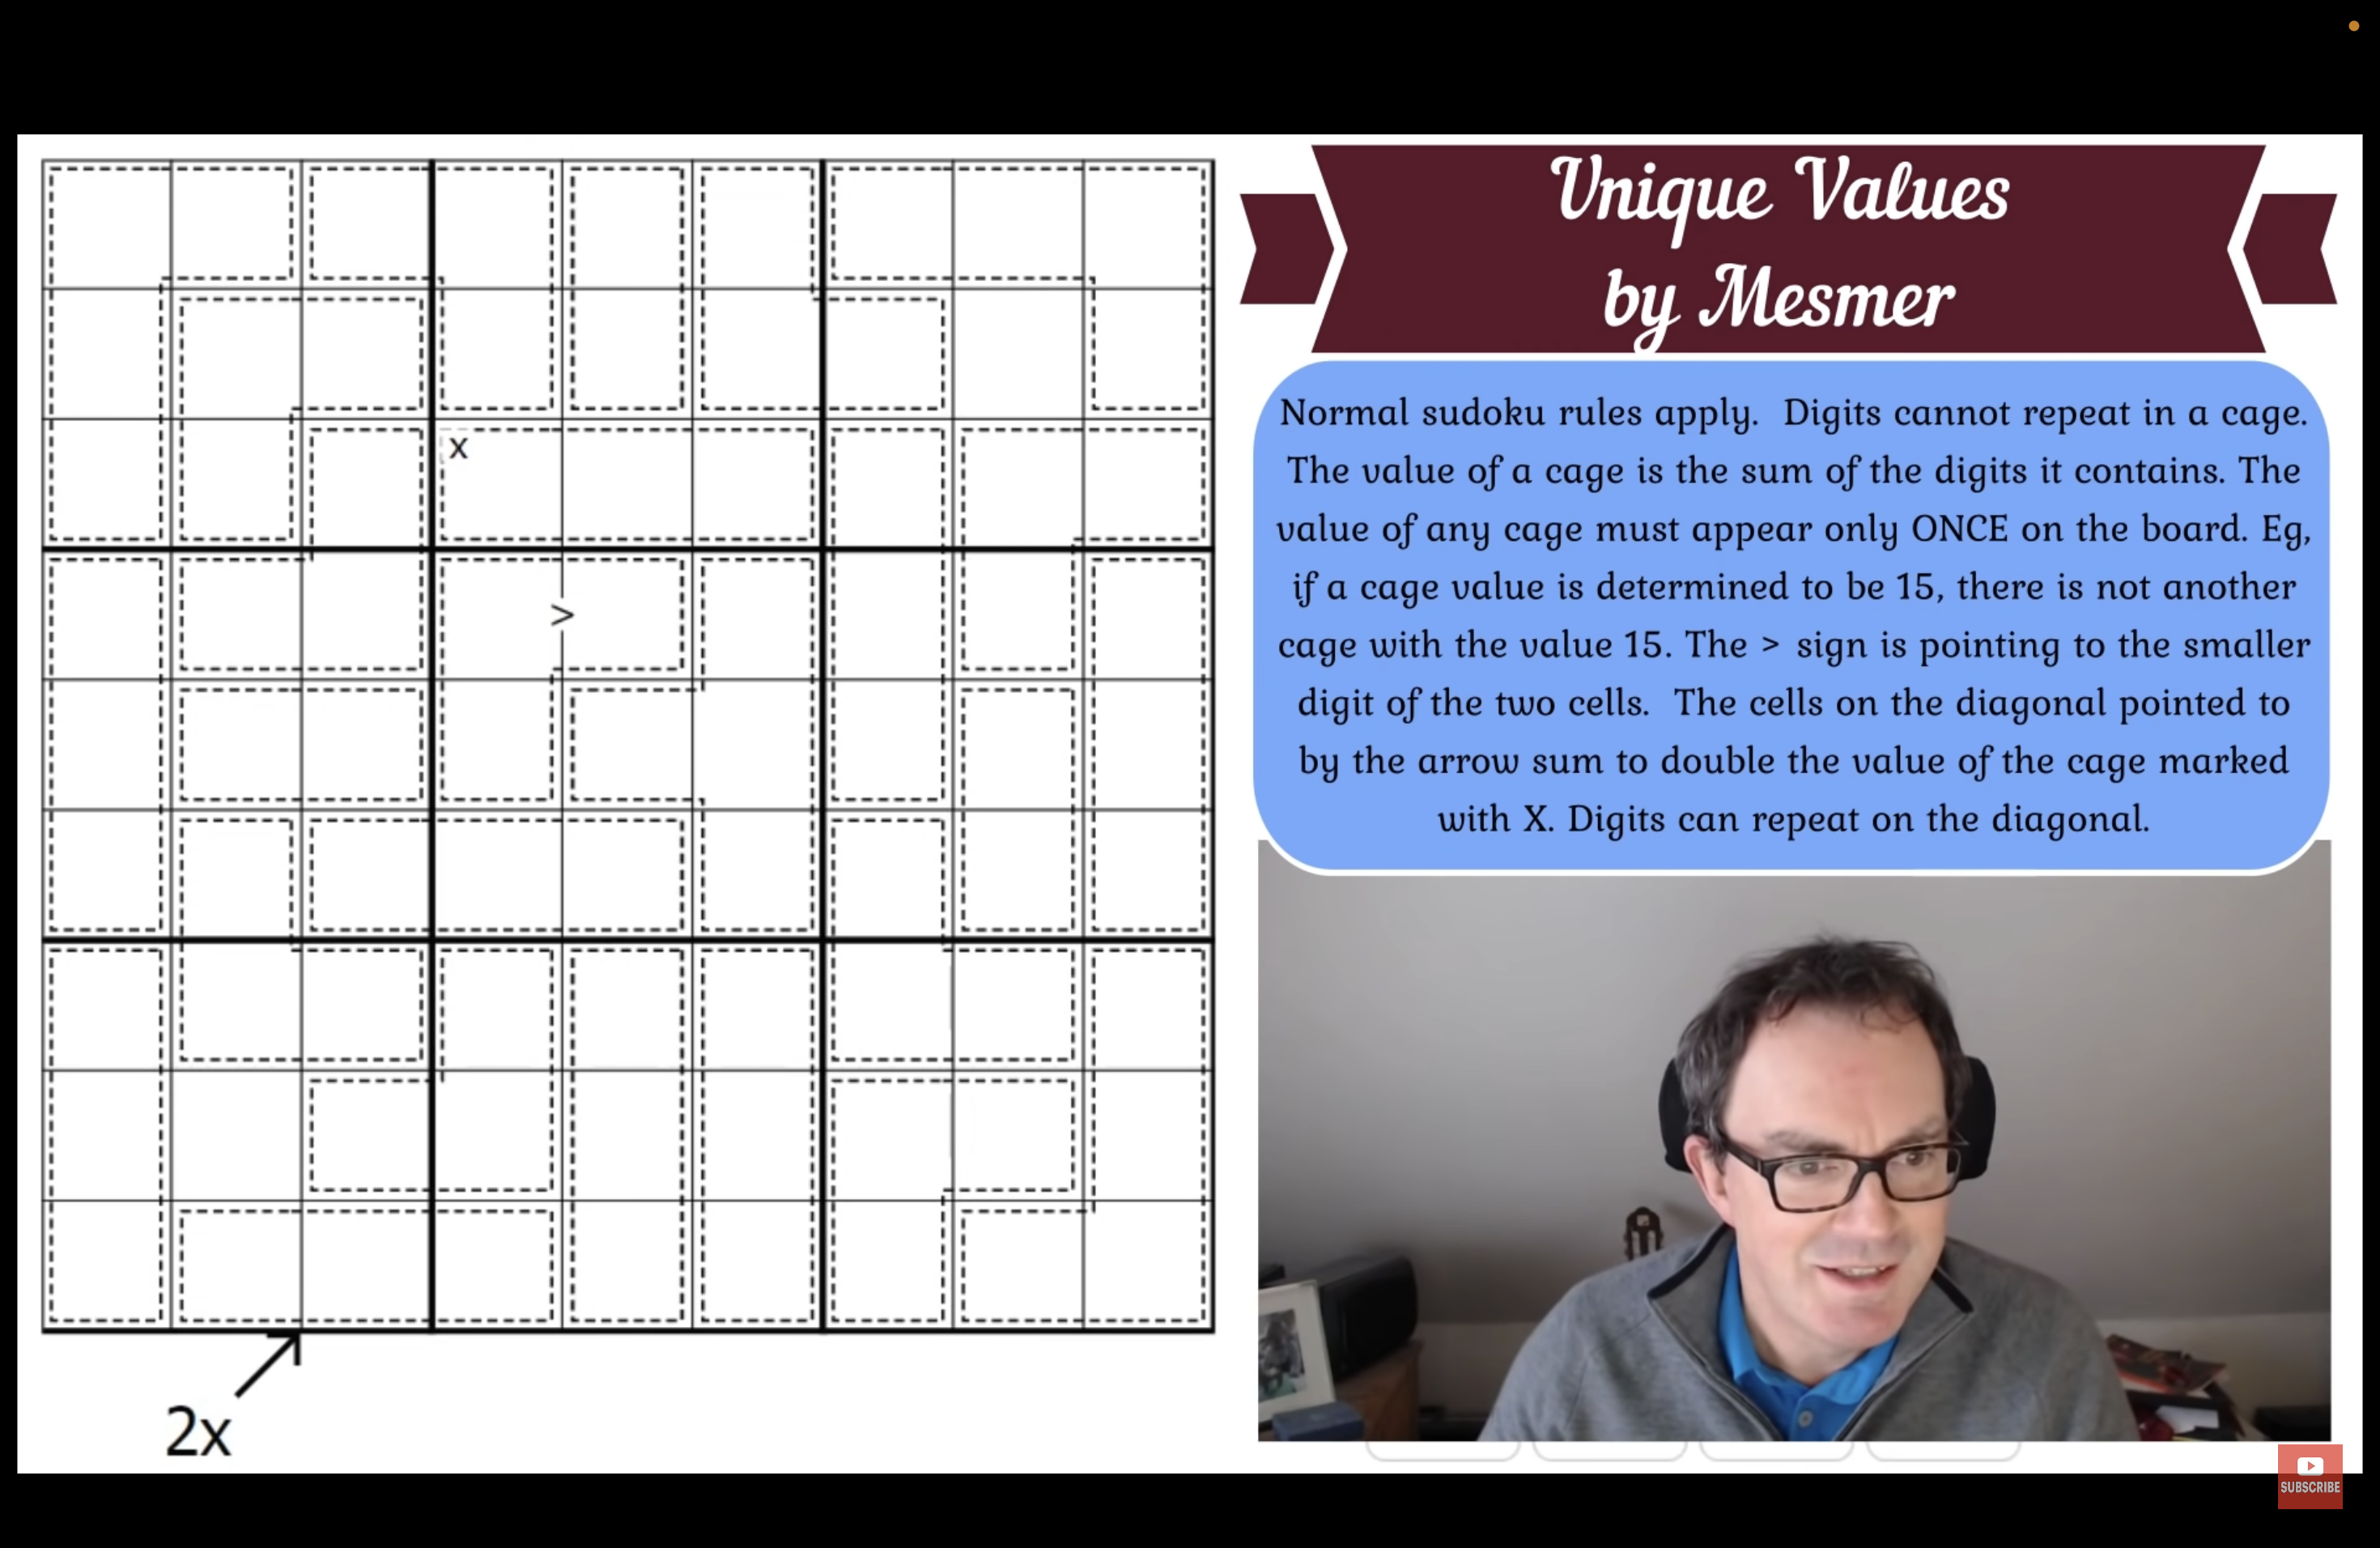
\includegraphics[scale=0.35]{puzzle2}
\end{center}
There are 3 cages of 2 cells, 19 cages of 3 cells, and 4 cages of 4 cells. The range of possible values are:
\begin{center}
\begin{tabular} {|c|c|c|}
\hline
\# of Cells & Minimum Value & Maximum Value\\
\hline
2 & $1+2=3$ & $8+9=17$\\
\hline
3 & $1+2+3=6$ & $7+8+9=24$\\
\hline
4 & $1+2+3+4=10$ & $6+7+8+9=30$\\
\hline
\end{tabular}
\end{center}
There are 19 possible values for 19 cages of 3 cells, so every single value must be used. Then, after excluding 6 to 24 from the range of values of cages of 2 cells, there are 3 possible values for 3 cages of 2 cells, so all of these must be used, too. Now the minimum value of the sum of all cages is sum of all integers from 3 to 28 which is $\frac{(3+28)(28-3+1)}{2} = 403$ when there are two cells in the entire grid that is not caged, and the sum of all numbers in a grid must be $\frac{9(1+9)}{2}\cdot9 = 405$. The sum of uncaged two cells cannot be less than 2, so the value of 4 cages of 4 cells must be 25 to 28 while the two uncaged cells are both 1. From here, I just eliminated possibilities and filled out the determined digits one by one until it was finished. Here's the completed version:
\begin{center}
\addtolength{\leftskip} {-2cm} % increase (absolute) value if needed
\addtolength{\rightskip}{-2cm}
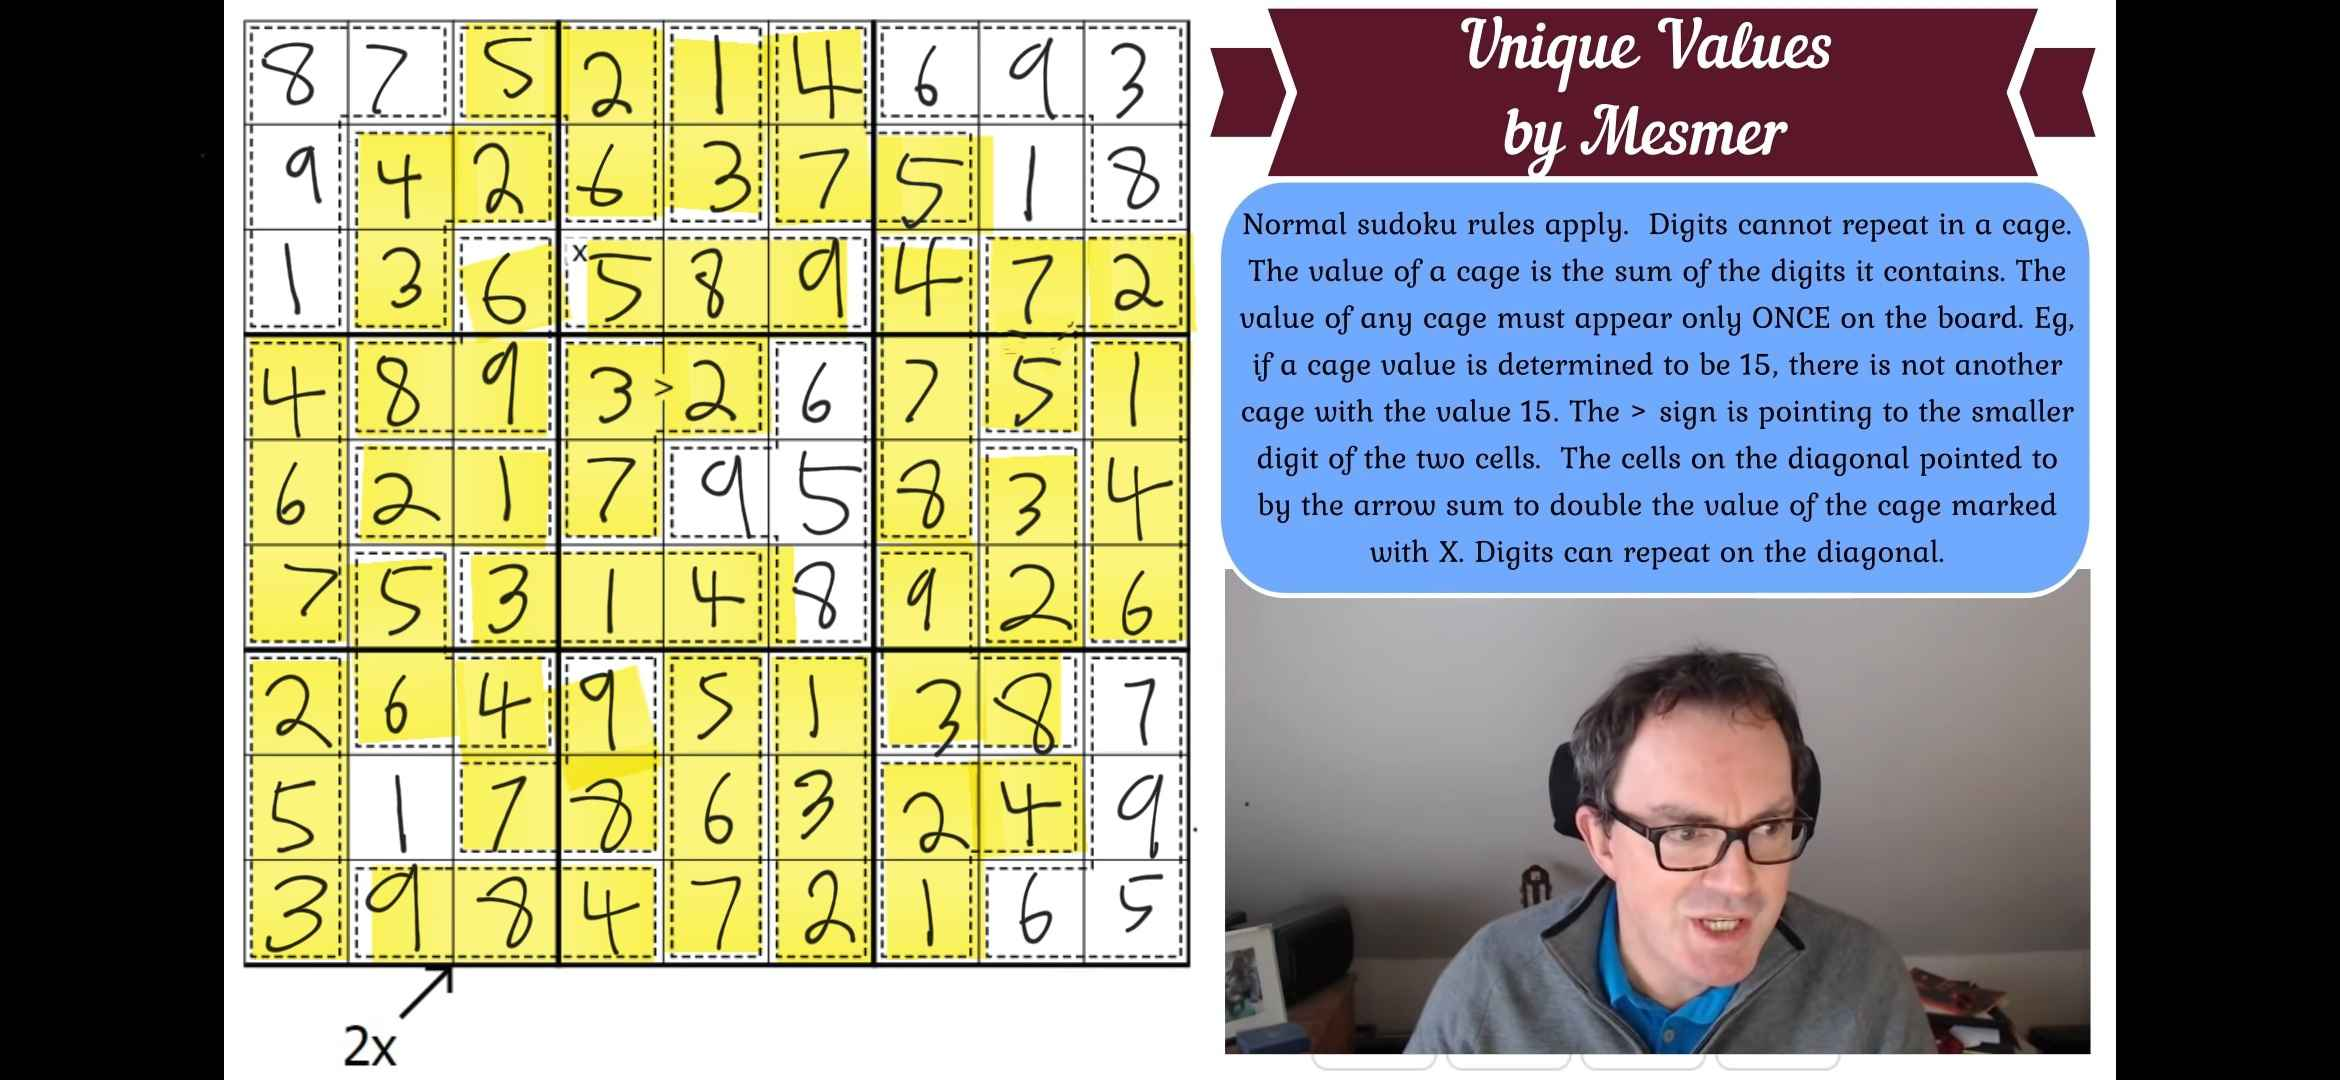
\includegraphics[scale=0.22]{puzzle2sln}
\end{center}
I have solved a total of three variants of sudoku introduced by the same YouTube channel, and they were all really fun. I will keep trying the fun-looking ones when I have spare time.
\section*{$\frac{\pi}{n} \sim \sin(\frac{\pi}{n})$}
\textbf{10/02/2024}\\
In an introductory assignment to Python turtle graphics, a drawing tool, I first made a function that draws a regular polygon with $n$ sides with each side length $l$. Then, I was told to make a function that draws a circle using the polygon function to draw a regular polygon with a lot of sides. However, I was only given a radius $r$ when I needed the length of each sides. I figured dividing the circumference of a circle by the number of sides will give me the length of each side, giving me this formula: \[l = 2 \cdot r \cdot \pi / n.\] However, the instruction told me to use this formula: \[l = 2 \cdot r \cdot \sin(\pi / n).\] I eventually figured out how to derive this formula.
\begin{center}
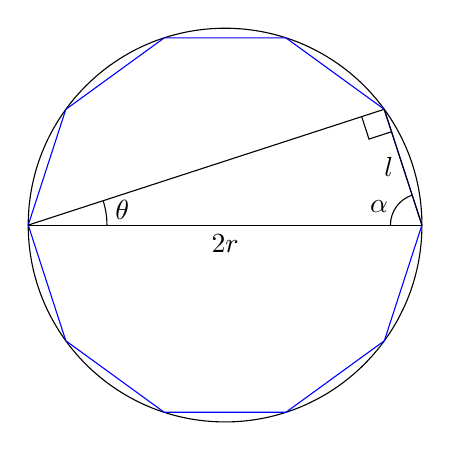
\begin{tikzpicture}
\draw circle(2.5cm);
\coordinate (A) at (-2.5,0);
\coordinate (B) at (2.5,0);
\coordinate (C) at (2.02,1.47);
\node[blue, regular polygon, regular polygon sides=10, minimum size=5cm, draw] {};
\draw (A) -- (B) node[below, midway]{$2r$};
\draw (A) -- (C);
\draw (B) -- (C) node[left, midway, shift={(0mm,0mm)}]{$l$};
\draw pic[draw,angle radius=1cm,"$\theta$" shift={(6mm,1mm)}] {angle=B--A--C};
\draw pic[draw,angle radius=4mm,"$\alpha$" shift={(-3.5mm,1mm)}] {angle=C--B--A};
\draw pic[draw,angle radius=3mm] {right angle=A--C--B};
\end{tikzpicture}
\end{center}
Draw a right triangle with its hypotenuse the diameter of the circle and one side being the side of the regular polygon. The angle opposed to the side $\theta$ is $\dfrac{\pi}{n}$.
\begin{eqnarray*}
\theta & = & \frac{\pi}{2} - \alpha\\
& = & \frac{\pi}{2} - \frac{1}{2} \cdot \text{(interior angle of regular polygon)}\\
& = & \frac{\pi}{2} - \frac{1}{2} \cdot \frac{\pi \cdot n - 2 \cdot \pi}{n}\\
& = & \frac{\pi}{n}\\
\end{eqnarray*}
From this, 
\begin{eqnarray*}
& \sin(\pi/n) = \dfrac{l}{2r}\\
\Leftrightarrow & l = 2 \cdot r \cdot \sin(\pi/n).
\end{eqnarray*}
Here, I couldn't find any flaw in logic for both formulas, so I wondered if $\sin(\pi/n)$ and $\pi/n$ were equal. However, I knew that cannot be the case, then I realized this is a special case where $n$ is supposed to be as big as possible. $\sin\left(\dfrac{\pi}{n}\right) = \dfrac{\pi}{n}$ holds true when $n$ approaches infinity. If $\sin\left(\dfrac{\pi}{n}\right) = \dfrac{\pi}{n}$, then $\dfrac{\sin\left(\dfrac{\pi}{n}\right)}{\dfrac{\pi}{n}} = 1$. We can write:
\[\lim_{n\rightarrow\infty} \dfrac{\sin\left(\dfrac{\pi}{n}\right)}{\dfrac{\pi}{n}} = 1\] 
Substitute $x = \dfrac{\pi}{n}$ which approaches 0 as $n$ approaches $\infty$.\\
\[\lim_{x\rightarrow0} \dfrac{\sin(x)}{x} = 1\]
Now, this was a familiar limit I had learned previously. It was cool to see how this limit can be shown geometrically.
\section*{Sum of Divisiors}
\textbf{10/04/2024}\\
\begin{quote}If sum of the divisors of $n$ (including $n$) is greater than $4n$, what is the lowest number of $n$'s prime divisors?\end{quote}
Write $n = p_1^{e_1}p_2^{e_2} \cdots p_k^{e_k}$ with each $p_i$ being a distinct prime factor of $n$. Say $S(n)$ represent the sum of all divisors of $n$, then \[S(n) = \left(\frac{p_1^{e_1+1}-1}{p_1-1}\right)\left(\frac{p_2^{e_2+1}-1}{p_2-1}\right)\cdots\left(\frac{p_k^{e_k+1}-1}{p_k-1}\right).\] Since $S(n) > 4n$, it follows that $\dfrac{S(n)}{n} > 4$.
\begin{eqnarray*}
\dfrac{S(n)}{n} & = & \dfrac{\left(\dfrac{p_1^{e_1+1}-1}{p_1-1}\right)\left(\dfrac{p_2^{e_2+1}-1}{p_2-1}\right)\cdots\left(\dfrac{p_k^{e_k+1}-1}{p_k-1}\right)}{p_1^{e_1}p_2^{e_2} \cdots p_k^{e_k}}\\
& = & \left(\frac{p_1^{e_1+1}-1}{p_1^{e_1}(p_1-1)}\right)\left(\frac{p_2^{e_2+1}-1}{p_2^{e_2}(p_2-1)}\right)\cdots\left(\frac{p_k^{e_k+1}-1}{p_k^{e_k}(p_k-1)}\right)\\
& = & \left(\dfrac{p_1-\dfrac{1}{p_1^{e_1}}}{p_1-1}\right)\left(\dfrac{p_2-\dfrac{1}{p_2^{e_2}}}{p_2-1}\right)\cdots\left(\dfrac{p_k-\dfrac{1}{p_k^{e_k}}}{p_k-1}\right)\\
\end{eqnarray*}
We can maximize the exponent of each prime factor to maximize $\dfrac{S(n)}{n}$:
\[
\left(\dfrac{p_1-\dfrac{1}{p_1^{e_1}}}{p_1-1}\right)\left(\dfrac{p_2-\dfrac{1}{p_2^{e_2}}}{p_2-1}\right)\cdots\left(\dfrac{p_k-\dfrac{1}{p_k^{e_k}}}{p_k-1}\right) < \left(\dfrac{p_1}{p_1-1}\right)\left(\dfrac{p_2}{p_2-1}\right)\cdots\left(\dfrac{p_k}{p_k-1}\right)
\]
The left side can be arbitrarily close to the right side since maximizing the exponents will cause $\dfrac{1}{p_i^{e_i}}$ to approach 0. Notice that $\dfrac{p_i}{p_i-1}$ decreases as $p_i$ increases, so we want each prime factor to be as small as possible. If the lowest number of $n$'s prime divisors is 3, then $S(n)/n$ is maximized when the prime divisors are 2, 3 and 5:
\[
\frac{S(n)}{n} < \frac{2}{1} \cdot \frac{3}{2} \cdot \frac{5}{4} = \frac{15}{4} < 4
\]
$S(n)/n$ can never reach 4. If the lowest number of $n$'s prime divisors is 4, then $S(n)/n$ is maximized when the prime divisors are 2, 3, 5 and 7:
\[
\frac{S(n)}{n} < \frac{2}{1} \cdot \frac{3}{2} \cdot \frac{5}{4} \cdot \frac{7}{6} = \frac{35}{8} > 4
\]
This means $S(n)/n$ can get arbitrarily close to $\dfrac{35}{8}$, which is bigger than 4. Thus, the lowest number of $n$'s prime divisors for the sum of the divisors of $n$ to be greater than $4n$ is 4.
\section*{Necessity and Sufficiency}
\textbf{10/08/2024}\\
While learning about logic, I came across how necessity and sufficiency can describe a conditional or implicational relationships. I kept confusing the two, so I am just reviewing them to make sure I understand.

Say $p, q$ are two arbitrary statements. A conditional statement made of them, "If $p$, then $q$" can be written as $p \rightarrow q$, and the truth table looks like the following:
\begin{center}
\begin{tabular}{|c|c|c|}
\hline
$p$ & $q$ & $p \rightarrow q$\\
\hline
T & T & T\\
\hline
T & F & F\\
\hline
F & T & T\\
\hline
F & F & T\\
\hline
\end{tabular}
\end{center}
If we say $p$ is necessary for $q$, that means if $q$ is true, then $p$ must be true. This corresponds to "if $q$, then $p$".
\[ p \text{ is necessary for } q \Leftrightarrow q \rightarrow p\]
If we say $p$ is sufficient for $q$, that means if $p$ is true, then $q$ will be true. This corresponds to "if $p$, then $q$".
\[ p \text{ is sufficient for } q \Leftrightarrow p \rightarrow q\]
\section*{Counting Multiples}
\textbf{10/11/2024}\\
\begin{quote}
How many positive multiples of 3 or 5 or 134 are there that are less than 2015?
\end{quote}
I solved this problem while preparing for the next week's Math Challengers meeting. At first, I simply counted using the inclusion-exclusion principle which generalizes the method of counting the size of union of multiple sets. Here's the principle:
\begin{quote}
To find the cardinality of the union of $n$ sets:
\begin{enumerate}
\item Include the cardinalities of the sets.
\item Exclude the cardinalities of the pairwise intersections.
\item Include the cardinalities of the triple-wise intersections.
\item Continue, until the cardinality of the $n$-tuple-wise intersection is included (if $n$ is odd) or excluded ($n$ even).
\end{enumerate}
\end{quote}
Cardinality refers to the size of a set, or the number of elements in a set. I applied this principle to the problem:
\begin{eqnarray*}
&&[\text{(\# of multiples of 3)} + \text{(\# of multiples of 5)} + \text{(\# of multiples of 134)}]\\
& - &[\text{(\# of multiples of $3\cdot5$)} + \text{(\# of multiples of $3\cdot134$)} + \text{(\# of multiples of $5\cdot134$)}]\\
& + &\text{(\# of multiples of $3\cdot5\cdot134$)}\\
& = &(671 + 402 + 15)\\
& - &(134 + 5 + 3)\\
& + &1\\
& = &947
\end{eqnarray*}
However, this method required too much calculations and took too long for a competition. I felt like there should be a better way. Then, I thought of the Euler's totient function $\phi(n)$ which counts the numbers less than $n$ that are co-prime with $n$. 
\begin{quote}
For each $p_i$ with $1 \leq i \leq k$ being distinct prime factors of $n$,
\[\phi(n) = n\left(1-\frac{1}{p_1}\right)\left(1-\frac{1}{p_2}\right)\cdots\left(1-\frac{1}{p_k}\right)\]
\end{quote}
Using a similar method, I counted the numbers less than 2010 that are not multiples of 3 or 5 or 134:
\[2010 \cdot \frac{2}{3} \cdot \frac{4}{5} \cdot \frac{133}{134} = 1064.\]
Subtracting from 2010, I get the number of multiples of 3 or 5 or 134 less than or equal to 2010:
\[2010 - 1064 = 946.\]
Now, only 2013 from 2011 to 2014 is a multiple of 3 or 5 or 134, so add one, getting the same answer of 947.

To generalize when and how to use this method, say the question asks you to find how many positive multiples of $m_1$, $m_2$, \dots, or $m_k$ $(m_i \leq n)$ are there that are less than $n$. You can use this method If 1 is the only common positive divisor of all of $m_i$, and if the product of all $m_i$, say $M$, is smaller than $n$. Then, find $x$, a multiple of $M$ that is smaller than but is the closest to $n$. Calculate
\[x\left(\frac{m_1-1}{m_1}\right)\left(\frac{m_2-1}{m_2}\right)\cdots\left(\frac{m_k-1}{m_k}\right)\]
to count the numbers that are not multiple of any $m_i$, then subtract from $x$ to count only the multiples. Now, count how many multiples are in the range from $x+1$ to $n-1$ using any methods. This can be quite useful.
\section*{Lockbox Submission}
\textbf{10/13/2024}\\
I submitted this problem with a little change for the lockbox:
\begin{quote}
$a, b, c$ are positive integers such that
\[\frac{1}{a}+\frac{1}{b}+\frac{1}{c}<1.\]
Prove that
\[\frac{1}{a}+\frac{1}{b}+\frac{1}{c}\leq\frac{41}{42}.\]
\end{quote}
This is from the problem of the week for the last year's COMC.

First, I assume $\dfrac{1}{a} \geq \dfrac{1}{b} \geq \dfrac{1}{c} \text{ or } (a\leq b\leq c)$ without loss of generality because of complete symmetry (You can always switch their order to satisfy the condition). I simply consider all the cases:
\pagebreak
\begin{tabbing}
\=$a=1$\=\\
\>\>$\dfrac{1}{a}+\dfrac{1}{b}+\dfrac{1}{c}\geq1$\=\\
\=$a=2$\=\\
\>\>$b<3$\=\\
\>\>\>$\dfrac{1}{a}+\dfrac{1}{b}+\dfrac{1}{c}\geq1$\=\\
\>\>$b=3$\=\\
\>\>\>$c<7$\=\\
\>\>\>\>$\dfrac{1}{a}+\dfrac{1}{b}+\dfrac{1}{c}\geq1$\=\\
\>\>\>$c\geq7$\=\\
\>\>\>\>$\dfrac{1}{a}+\dfrac{1}{b}+\dfrac{1}{c}\leq\dfrac{1}{2}+\dfrac{1}{3}+\dfrac{1}{7}=\dfrac{41}{42}\leq\dfrac{41}{42}$\=\\
\>\>$b=4$\=\\
\>\>\>$c<5$\=\\
\>\>\>\>$\dfrac{1}{a}+\dfrac{1}{b}+\dfrac{1}{c}\geq1$\=\\
\>\>\>$c\geq5$\=\\
\>\>\>\>$\dfrac{1}{a}+\dfrac{1}{b}+\dfrac{1}{c}\leq\dfrac{1}{2}+\dfrac{1}{4}+\dfrac{1}{5}=\dfrac{19}{20}\leq\dfrac{41}{42}$\=\\
\>\>$b\geq5$\=\\
\>\>\>$\dfrac{1}{a}+\dfrac{1}{b}+\dfrac{1}{c}\leq\dfrac{1}{2}+\dfrac{1}{5}+\dfrac{1}{5}=\dfrac{9}{10}\leq\dfrac{41}{42}$\=\\
\=$a=3$\=\\
\>\>$b=3$\=\\
\>\>\>$c<4$\=\\
\>\>\>\>$\dfrac{1}{a}+\dfrac{1}{b}+\dfrac{1}{c}\geq1$\=\\
\>\>\>$c\geq4$\=\\
\>\>\>\>$\dfrac{1}{a}+\dfrac{1}{b}+\dfrac{1}{c}\leq\dfrac{1}{3}+\dfrac{1}{3}+\dfrac{1}{4}=\dfrac{11}{12}\leq\dfrac{41}{42}$\=\\
\>\>$b\geq4$\=\\
\>\>\>$\dfrac{1}{a}+\dfrac{1}{b}+\dfrac{1}{c}\leq\dfrac{1}{3}+\dfrac{1}{4}+\dfrac{1}{4}=\dfrac{5}{6}\leq\dfrac{41}{42}$\=\\
\=$a\geq4$\=\\
\>\>$\dfrac{1}{a}+\dfrac{1}{b}+\dfrac{1}{c}\leq\dfrac{1}{4}+\dfrac{1}{4}+\dfrac{1}{4}=\dfrac{3}{4}\leq\dfrac{41}{42}$\=\\
\end{tabbing}
You can see that the inequality we are trying to prove is true or the initial condition is false in every case, so it is proven.
\section*{Lockbox Submission Review}
\textbf{10/16/2024}\\
For the problem I submitted related to calculating a probability of basketball shots (Putnam 2002 B1), I found out a more generalized solution as I read the official solution. It claims that the probability of having made any number of shots from 1 to $n-1$ out of $n$ shots are all equal to $\dfrac{1}{n-1}$. This can be proved by induction on $n$.

Let $P(i, n)$ denote the probability of hitting $i$ out of $n$ shots.\\
Claim: $P(i, n) = \dfrac{1}{n-1}$ for $1 \leq i \leq n-1$\\
Base case: $P(1, 2) = 1 = \dfrac{1}{2-1}$. This is trivial.\\
Suppose the claim is true for $n=k$. That is, . \\
Then, the probability of hitting $i$ out of $k+1$ shots ($2 \leq i \leq k-1$) is: 
\begin{eqnarray*}
& P(i, k+1)\\
= & P(i, k) \cdot \text{(misses the $k+1$th shot)} + P(i-1, k) \cdot \text{(hits the $k+1$th shot)}\\
= & P(i, k) \cdot \dfrac{k-i}{k} + P(i-1, k) \cdot \dfrac{i-1}{k}\\
= & \dfrac{1}{k-1} \cdot \dfrac{k-i}{k} + \dfrac{1}{k-1} \cdot \dfrac{i-1}{k}\\
= & \dfrac{1}{k-1} \cdot \left(\dfrac{k-i}{k} + \dfrac{i-1}{k}\right)\\
= & \dfrac{1}{k-1} \cdot \dfrac{k-1}{k}\\
= & \dfrac{1}{k}.
\end{eqnarray*}
If $i=1$:
\begin{eqnarray*}
& P(1, k+1)\\
= & P(1, k) \cdot \text{(misses the $k+1$th shot)}\\
= & P(1, k) \cdot \dfrac{k-1}{k}\\
= & \dfrac{1}{k-1} \cdot \dfrac{k-1}{k}\\
= & \dfrac{1}{k}.
\end{eqnarray*}
If $i=k$:
\begin{eqnarray*}
& P(k, k+1)\\
= & P(k-1, k) \cdot \text{(hits the $k+1$th shot)}\\
= & P(k-1, k) \cdot \dfrac{k-1}{k}\\
= & \dfrac{1}{k-1} \cdot \dfrac{k-1}{k}\\
= & \dfrac{1}{k}.
\end{eqnarray*}
Thus, the claim is also true for $n=k+1$. This completes the proof, so the probability of hitting exactly 50 of 100 shots is 1/99.
\section*{COMC 2011 C4}
\textbf{10/27/2024}\\
I encountered this question while preparing for the upcoming Canadian Open Mathematics Challenge.
\begin{quote}
Let $f(x) = x^2 - ax + b$, where $a$ and $b$ are positive integers.
\begin{enumerate} [a)]
\item Suppose $a=2$ and $b=2$. Determine the set of real roots of $f(x) - x$, and the set of real roots of $f(f(x)) - x$. 
\item Determine the number of pairs of positive integers $(a, b)$ with $1 \leq a,b \leq 2011$ for which every root of $f(f(x)) -x$ is an integer.
\end{enumerate}
\end{quote}
Here is how I solved this:
\begin{enumerate} [a)]
\item Solve $f(x) - x = 0$.
\begin{eqnarray*}
(x^2 - 2x + 2) - x &=& 0\\
x^2 - 3x + 2 &=& 0\\
(x - 2) (x - 1) &=& 0\\
x &=& 1, 2
\end{eqnarray*}
Notice that $f(x) - x = 0 \Leftrightarrow f(x) = x$, so the roots of this equation return itself when put inside $f(x)$. $f(f(x)) - x = 0 \Leftrightarrow f(f(x)) = x$, so the roots of the first equation satisfy this equation as well. Now, I can factor the known roots out from $f(f(x)) - x$. 
\begin{eqnarray*}
f(f(x)) - x &=& (x^2 - 2x + 2)^2 - 2(x^2 - 2x + 2) + 2 - x\\
&=& (x^4 + 4x^2 + 4 - 4x^3 + 4x^2 -8x) + (- 2x^2 + 4x - 4) + 2 - x\\
&=& x^4 -4x^3 + 6x^2 - 5x + 2
\end{eqnarray*}
Divide $f(f(x)) - x$ by $(x-1)$ and $(x-2)$ using synthetic division.
\begin{center}
\begin{tabular} {cccccc}
\multicolumn{1}{c|} 1 & 1 & -4 & 6 & -5 & 2\\
\multicolumn{1}{c|} {}&&1&-3&3&-2\\
\cline{2-6}
\multicolumn{1}{c|} 2&1&-3&3&-2&0\\
\multicolumn{1}{c|} {}&&2&-2&2&\\
\cline{2-6}
&1&-1&1&0&\\
\end{tabular}
\end{center}
\[f(f(x)) - x = (x-1)(x-2)(x^2-x+1).\]
$x^2 - x + 1$ does not have a real root since its discriminant is negative: $b^2 - 4ac = (-1)^2 - 4(1)(1) = -3 < 0.$ Thus, the sets of real roots of $f(x) - x$ and $f(f(x)) - x$ are both \{1, 2\}.
\item From a), I know $f(x) - x$ divides $f(f(x)) - x$.
\begin{eqnarray*}
f(f(x)) - x &=& (x^2-ax+b)^2-a(x^2-ax+b)+b - x\\
&=& (x^4+a^2x^2+b^2-2ax^3+2bx^2-2abx)+(-ax^2+a^2x-ab)+b - x\\
&=& x^4 - 2ax^3 + (a^2+2b-a)x^2 + (-2ab+a^2-1)x + b^2 + b - ab
\end{eqnarray*}
Divide $f(f(x)) - x$ by $f(x) - x = x^2 - (a+1)x + b$.
\begin{center}
\addtolength{\leftskip} {-2cm} % increase (absolute) value if needed
\addtolength{\rightskip}{-2cm}
\begin{tabular} {cccccc}
&$x^2$&$(1-a)x$&$(b-a+1)$&&\\
\cline{2-6}
\multicolumn{1}{c|} {$x^2 - (a+1)x + b$} & $x^4$ & $-2ax^3$ & $(a^2+2b-a)x^2$ & $(-2ab+a^2-1)x$ & $b^2 + b - ab$\\
& $x^4$ & $-(a+1)x^3$ & $bx^2$ &&\\
\cline{2-4}
 && $(1-a)x^3$ & $(a^2+b-a)x^2$ &&\\
&& $(1-a)x^3$ & $(a^2-1)x^2$ &$(b-ab)x$&\\
\cline{3-5}
&&&$(b-a+1)x^2$&$(a^2-ab-b-1)x$&\\
&&&$(b-a+1)x^2$&$(a^2-ab-b-1)x$&$b^2 + b - ab$\\
\cline{4-6}
&&&&&0
\end{tabular}
\end{center}
\[f(f(x)) - x = (x^2 - (a+1)x + b)(x^2+(1-a)x + b-a+1)\]
For every root of $f(f(x)) - x$ to be an integer, every root of these two quadratic factors must be an integer. This means the discriminants of both quadratics must be perfect squares. The two discriminants are:
\[(a+1)^2 - 4b = a^2 + 2a - 4b + 1\]
\[(1-a)^2 - 4(b-a+1) = a^2 + 2a - 4b - 3\]
They differ by 4, and the only two perfect squares with a difference of 4 are 0 and 4. Therefore, $a^2 + 2a - 4b - 3 = 0$.
\begin{eqnarray*}
a^2 + 2a - 4b - 3 &=& 0\\
a(a+2) &=& 4b + 3
\end{eqnarray*}
If $a$ is an even integer, $a(a+2)$ becomes a multiple of 4 since $2k(2k+2)=4(k^2+k)$, so no integer $b$ satifies the equation.

If $a$ is an odd integer, $a(a+2) = (2k+1)(2k+3) = 4k^2 + 8k + 3 = 4(k^2 + 2k) + 3$, so $a=2k+1$ and $b=k^2+2k$.

Now count the number of integer $k$ that satifies $1 \leq a,b \leq 2011$. $k \geq 1$ since $b = 0$ if $k = 0$. $b$ grows faster than $a$, so check the bound only with $b$. If $k=43$, $b=1935$, and if $k=44$, $b=2024$. Thus, $1 \leq k \leq 43$. There are 43 pairs of postive integers (a, b) with $1 \leq a, b \leq 2011$ for which every root of $f(f(x)) - x$ is an integer.
\end{enumerate}
\section*{COMC 2024 B4}
\textbf{11/02/2024}\\
Here is a problem from this year's COMC that I thought was interesting.
\begin{quote}
Initially, the integer 80 is written on a blackboard. At each step, the integer $x$ on the
blackboard is replaced with an integer chosen uniformly at random among $[0, x-1]$, unless
$x = 0$, in which case it is replaced by an integer chosen uniformly at random among $[0, 2024]$.
Let $P(a, b)$ be the probability that after $a$ steps, the integer on the board is $b$. Determine
\[ \lim_{a \rightarrow \infty} \frac{P(a, 80)}{P(a, 2024)}\]
\end{quote}
The official solution is not out yet, but here is how I solved it:

Consider $P(a, 2024)$. For the integer to be 2024 after $a$ steps, the integer must be 0 after $a-1$ steps, and 2024 must be chosen uniformly at random among $[0, 2024]$ (2025 integers).
\[P(a, 2024) = P(a-1, 0) \cdot \frac{1}{2025}\]
Now, consider $P(a, 2023)$. There are two ways for the integer to be 2023 after $a$ steps. 2023 can be chosen among $[0, 2024]$ after the integer on the previous step was 0, or 2023 can be chosen among $[0, 2023]$ after the integer on the previous step was 2024.
\[P(a, 2023) = P(a-1, 0) \cdot \frac{1}{2025} + P(a-1, 2024) \cdot \frac{1}{2024}\]
Since $\displaystyle \lim_{a \rightarrow \infty} a = \lim_{a \rightarrow \infty} a-1$, these two limits are also equivalent. \[ \lim_{a \rightarrow \infty} P(a, 2024) = \lim_{a \rightarrow \infty} P(a-1, 2024)\]
We are interested in only interested in $P(a, b)$ as $a$ goes to infinity, so assume all $P(a, b)$ are $\lim_{a \rightarrow \infty} P(a, b)$.
\begin{eqnarray*}
P(a, 2023) &=& P(a-1, 0) \cdot \dfrac{1}{2025} + P(a-1, 2024) \cdot \dfrac{1}{2024}\\
 &=& P(a-1, 0) \cdot \dfrac{1}{2025} + P(a-1, 0) \cdot \dfrac{1}{2025} \cdot \dfrac{1}{2024}\\
 &=& P(a-1, 0) (\dfrac{1}{2025} + \dfrac{1}{2025} \cdot \dfrac{1}{2024})\\
 &=& P(a-1, 0) \cdot \dfrac{1}{2024}.\\
 \end{eqnarray*}
 Similarly, 
\begin{eqnarray*}
P(a, 2022) &=& P(a-1, 0) \cdot \dfrac{1}{2025} + P(a-1, 2024) \cdot \dfrac{1}{2024} + P(a-1, 2023) \cdot \dfrac{1}{2023}\\
 &=& P(a-1, 0) \cdot \dfrac{1}{2025} + P(a-1, 0) \cdot \dfrac{1}{2025} \cdot \dfrac{1}{2024} + P(a-1, 0) \cdot \dfrac{1}{2024} \cdot \dfrac{1}{2023}\\
 &=& P(a-1, 0) (\dfrac{1}{2025} + \dfrac{1}{2025} \cdot \dfrac{1}{2024} + \dfrac{1}{2024} \cdot \dfrac{1}{2023})\\
 &=& P(a-1, 0) \cdot \dfrac{1}{2023}.\\
\end{eqnarray*}
We can notice that $\displaystyle \lim_{a \rightarrow \infty} P(a, b) = P(a-1, 0) \cdot \frac{1}{b+1}$. Now prove it by induction:

Let $S(n): \displaystyle \lim_{a \rightarrow \infty} P(a, n) = P(a-1, 0) \cdot \frac{1}{n+1}$.\\
$\displaystyle S(2024): \lim_{a \rightarrow \infty} P(a, 2024) = P(a-1, 0) \cdot \dfrac{1}{2025}$ as shown before. $S(2024)$ is true.
Assume $S(k+1), S(k+2), \dots , S(2024)$ are true, and consider $S(k): \displaystyle \lim_{a \rightarrow \infty} P(a, k) = P(a-1, 0) \cdot \frac{1}{k+1}$ for $0 \leq k \leq 2024$.
\begin{eqnarray*}
\displaystyle P(a, k) &=& P(a-1, 0) \cdot \frac{1}{2025} + \sum_{i=k+1}^{2024} P(a-1, i) \cdot \frac{1}{i}\\
\displaystyle &=& P(a-1, 0) (\frac{1}{2025} + \sum_{i=k+1}^{2024} \frac{1}{i+1} \cdot \frac{1}{i})\\
\displaystyle &=& P(a-1, 0) \cdot \frac{1}{k+1}\\
\end{eqnarray*}
$[S(k+1) \wedge S(k+2) \wedge \cdots \wedge S(2024)] \Rightarrow S(k).$\\
By the Principle of Mathematical Induction, $\displaystyle \lim_{a \rightarrow \infty} P(a, n) = P(a-1, 0) \cdot \frac{1}{n+1}$ for all $0 \leq n \leq 2024$.

Now, the desired limit can be evaluated.
\[\lim_{a \rightarrow \infty} \frac{P(a, 80)}{P(a, 2024)} = \lim_{a \rightarrow \infty} \frac{\frac{1}{81}}{\frac{1}{2025}} = \frac{2025}{81} = 25.\]
\pagebreak
\section*{AMC 12A 2024 Problem 17}
\textbf{11/09/2024}\\
A fun problem I wanted to share from this year's AMC 12.
\begin{quote}
Integers $a$, $b$, and $c$ satisfy $ab + c = 100$, $bc + a = 87$, and $ca + b = 60$. What is $ab + bc + ca$?
\begin{enumerate} [A)]
\item 212
\item 247
\item 258
\item 276
\item 284
\end{enumerate}
\end{quote}
This is how I solved it:
\begin{center}
\begin{tabular} {ccc}
(1)&$ab + c = 100$&\\
(2)&$bc + a = 87$&\\
(3)&$ca + b = 60$&\\
(4)&$ab + c + bc + a = 100 + 87$&(1)+(2)\\
$\Leftrightarrow$&$(a+c)(b+1) = 187$&\\
(5)&$bc + a + ca + b = 87 + 60$&(2)+(3)\\
$\Leftrightarrow$&$(a+b)(c+1) = 147$&\\
(6)&$ab + c + ca + b = 100 + 60$&(1)+(3)\\
$\Leftrightarrow$&$(b+c)(a+1) = 160$&\\
\end{tabular}
\end{center}
Notice that in all (4), (5), and (6), the multiplicands add up to $a+b+c+1$. Since $187 = 11 \cdot 17$ and both factors are prime, 11 + 17 = 28 has to be the sum of multiplicands. $147 = 21 \cdot 7$ and $160 = 20 \cdot 8$, so 28 does work. Now $ab + bc + ca = ab + bc + ca - (a + b + c) = 100 + 87 + 60 - (28 - 1) = 220$, but 220 is not one of the multiple choices. 

Here, I realized that the sum can be negative, with $187 = -11 \cdot -17, 147 = -21 \cdot -7$, and $160 = -20 \cdot -8$. Letting the sum equal -28, $ab + bc + ca = ab + bc + ca - (a + b + c) = 100 + 87 + 60 - (-28 - 1) = 276$. The answer is D.
\section*{Number of Transitive Relations}
\textbf{11/16/2024}\\
I was asked to find the number of transitive relations in a set with 3 elements. A relation $R$ is a set of ordered pairs $(a, b)$ which means $a$ is related to $b$ (does not mean $b$ is related to $a$). A transitive relation $R$ is a relation where $(a, b) \in R$ and $(b, c) \in R$ implies $(a, c) \in R$ as well. A relation in a set with 3 elements (say $a, b, c$) is a subset of
\begin{eqnarray*}
\{&(a, a), (a, b), (a, c)&\\
&(b, a), (b, b), (b, c)&\\
&(c, a), (c, b), (c, c)&\}.
\end{eqnarray*}
It was way harder than I expected. At first, I tried to come up with a combinatoric way of representing it, but I failed. After trying and thinking for a long time, I decided to analyze it case by case, separating the cases by the number of $(a, b)$ with $a \neq b$ in the relation.\\
\begin{enumerate}
\item No $(a, b)$ with $a \neq b$ in $R$.\\
There are 3 $(a, a)$ that can be either included or not.\\
$\therefore 2^3=8$ relations.\\
\item 1 $(a, b)$ with $a \neq b$ in $R$.\\
6 choices for $(a, b)$ with $a \neq b$, then any $(a, a)$ can be included or not.\\
$\therefore 6 \cdot 2^3 = 48$ relations.\\
\item 2 $(a, b)$ with $a \neq b$ in $R$.\\
1) Either $(a, b), (a, c)$ or $(b, a), (c, a)$, and there are 3 choices for $a$. Then, any $(a, a)$ can be included or not.\\
2) $(a, b), (b, a), (a, a), (b, b)$, and there are 3 choices for $a, b$ (unordered). Then, $(c, c)$ can be included or not.\\
$\therefore 2 \cdot 3 \cdot 2^3 + 3 \cdot 2= 48 + 6 = 54$ relations.\\
\item 3 $(a, b)$ with $a \neq b$ in $R$.\\
6 choices for $(a, b), (b, c), (a, c)$, and any $(a, a)$ can be included or not.\\
$\therefore 6 \cdot 2^3 = 48$ relations.\\
\item 4 $(a, b)$ with $a \neq b$ in $R$.\\
1) Three choices for $(a, b), (b, c), (a, c), (b, a), (a, a), (b, b)$, and $(c, c)$ can be included or not.\\
2) Three choices for $(a, b), (b, c), (a, c), (c, b), (b, b), (c, c)$, and $(a, a)$ can be included or not.\\
$\therefore 3 \cdot 2 + 3 \cdot 2 = 12$ relations.\\
\item 5 $(a, b)$ with $a \neq b$ in $R$.\\
If $(a, b)$ is not in $R$, $(a, c), (c, b)$ are in $R$ so $(a, b)$ must be in $R$. None.\\
$\therefore 0$ relation.\\
\item 6 $(a, b)$ with $a \neq b$ in $R$.\\
All $(a, b)$ are included, and all $(a, a)$ must be included as well since $(a, b), (b, a)$ are in $R$.\\
$\therefore 1$ relation.\\
\end{enumerate}
In total, there are $8 + 48 + 54 + 48 + 12 + 0 + 1 = 171$ transitive relations.
\section*{Making Prime with Prime}
\textbf{01/05/2025}
\begin{quote}
Find all prime numbers that can be written as $p^q+q^p$ with primes $p, q$.
\end{quote}
I saw this problem on \href{https://youtu.be/a_jRo2_scLI}{YouTube}, and tried to solve it.

First, the smallest possible value of $p^q + q^p$ is $2^2 + 2^2 = 8$, so $p^q + q^p \geq 8$. Thus, it must be odd for it to be a prime number. If $p$ and $q$ have the same parity, then $p^q + q^p$ is an even number, so $p$ and $q$ must have different parity. 2 is the only even prime, so 2 must be one of them. $p$ and $q$ are interchangeable, so say $p$ is 2 and $q$ is an odd prime.

Now, we find all prime numbers that can be written as $2^q + q^2$ with an odd prime $q$. Consider the expression modulo 3. $2^q = (-1)^q \text{ (mod } 3)= -1 \text{ (mod } 3)$ since $q$ is odd.
\begin{itemize}
\item If $q = 1$ (mod 3), $q^2 = 1$ (mod 3) $\Rightarrow 2^q + q^2 = -1 + 1$ (mod 3) = 0 (mod 3).
\item If $q = 2$ (mod 3) = $-1$ (mod 3), $q^2 = 1$ (mod 3) $\Rightarrow 2^q + q^2 = -1 + 1$ (mod 3) = 0 (mod 3).
\item If $q = 0$ (mod 3), $q^2 = 0$ (mod 3) $\Rightarrow 2^q + q^2 = -1 + 0$ (mod 3) = -1 (mod 3).
\end{itemize}
Thus, $q$ must be 0 (mod 3) or $2^q + q^2$ will be a multiple of 3 (greater than 8) which is not prime. The only prime number that is 0 (mod 3) is 3, so consider $2^3 + 3^2 = 17$. 17 is prime, and we conclude that it is the only prime that can be written as $p^q + q^p$ with primes $p, q$. 
\section*{AM-GM Inequality}
\textbf{01/18/2025}
\begin{quote}
Let $a, b, c$ be real numbers, which are not all equal, such that
\[a + b + c = \frac{1}{a} + \frac{1}{b} + \frac{1}{c} = 3.\]
Prove that at least one of $a, b, c$ is negative.
\end{quote}
This problem can be proved easily using the inequality of arithmetic and geometric means which states that the arithmetic mean of non-negative real numbers is equal to or greater than the geometric mean of the same numberes. For two numbers $x$ and $y$, that is \[\frac{x+y}{2} \geq \sqrt{xy}.\] 
If $y=\dfrac{1}{x}$, 
\begin{eqnarray*}
&\dfrac{x+\dfrac{1}{x}}{2} &\geq \sqrt{x \cdot \dfrac{1}{x}}\\
\Rightarrow &x + \dfrac{1}{x} &\geq 2.
\end{eqnarray*}
We notice that $a + \dfrac{1}{a} + b + \dfrac{1}{b} + c + \dfrac{1}{c} = 6$. Suppose $a, b, c$ are all non-negative, then each $a + \dfrac{1}{a}, b + \dfrac{1}{b}, c + \dfrac{1}{c}$ are equal to or greater than 2. They must sum to 6, so they all have to equal to 2. $x+\dfrac{1}{x} = 2$ if and only if $x=1$, so $a=b=c=1$. However, $a, b, c$ are all different, so we reach a contradiction. At least one of $a, b, c$ has to be negative.
\section*{$\sqrt{2}$}
\textbf{01/22/2025}
\begin{quote}
Prove that $\sqrt{2}$ is always between $\dfrac{a}{b}$ and $\dfrac{a+2b}{a+b}$ for positive integers $a, b$. Which one is it closer to?
\end{quote}
This problem taught me an interesting way to show if a number is in an interval. If $x$ is between $A$ and $B$, then $(x-A)(x-B)$ will always be negative since $(x-A)$ and $(x-B)$ will have a opposite sign. If $x$ is outside the interval, they will have the same sign, so the expression will be positive.

Using this, we check the sign of $(\sqrt{2}-\dfrac{a}{b})(\sqrt{2}-\dfrac{a+2b}{a+b})$.
\begin{eqnarray*}
&(\sqrt{2}-\dfrac{a}{b})(\sqrt{2}-\dfrac{a+2b}{a+b})\\
=&(\dfrac{\sqrt{2}b-a}{b})(\dfrac{\sqrt{2}a+\sqrt{2}b-a-2b}{a+b})\\
=&(\dfrac{\sqrt{2}b-a}{b})(\dfrac{(\sqrt{2}-1)a+(\sqrt{2}-2)b}{a+b})\\
=&(\dfrac{\sqrt{2}b-a}{b})(\dfrac{(\sqrt{2}-1)a-(\sqrt{2}-1)\sqrt{2}b}{a+b})\\
=&(\dfrac{\sqrt{2}b-a}{b})(\dfrac{(\sqrt{2}-1)(a-\sqrt{2}b)}{a+b})\\
=&-\dfrac{(\sqrt{2}b-a)^2(\sqrt{2}-1)}{(b)(a+b)}
\end{eqnarray*}
$(\sqrt{2}b-a)^2$ and $\sqrt{2}-1$ are positive, and $b$ and $a+b$ are positive as well since we know $a$ and $b$ are positive. Thus, $(\sqrt{2}-\dfrac{a}{b})(\sqrt{2}-\dfrac{a+2b}{a+b})$ is negative and $\sqrt{2}$ is always between $\dfrac{a}{b}$ and $\dfrac{a+2b}{a+b}$ for positive integers $a, b$.

 Now, to see which one it is closer to, we check if $\dfrac{|\sqrt{2}-\dfrac{a}{b}|}{|\sqrt{2}-\dfrac{a+2b}{a+b}|}$ is always bigger than or smaller than 1. If it's bigger than 1, that means $\sqrt{2}$ is closer to $\dfrac{a+2b}{a+b}$, and otherwise if it's smaller than 1.
\begin{eqnarray*}
&\dfrac{|\sqrt{2}-\dfrac{a}{b}|}{|\sqrt{2}-\dfrac{a+2b}{a+b}|}\\\\
=&\left|\dfrac{\dfrac{\sqrt{2}b-a}{b}}{\dfrac{(\sqrt{2}-1)(a-\sqrt{2}b)}{a+b}}\right|\\\\
=&\left|\dfrac{\dfrac{1}{b}}{\dfrac{\sqrt{2}-1}{a+b}}\right|\\\\
=&\left|\dfrac{a+b}{(\sqrt{2}-1)b}\right|\\\\
=&\left|\dfrac{(\sqrt{2}+1)(a+b)}{b}\right|\\\\
\end{eqnarray*}
Since $\sqrt{2}+1>1$ and $a$ is positive, the absolute value is always greater than 1. Thus, $\sqrt{2}$ is always closer to $\dfrac{a+2b}{a+b}$ than $\dfrac{a}{b}$. 
\section*{$a^2 + b^2 = c^2$}
\textbf{01/29/2025}
\begin{quote}
How many pairs $(x, y)$ of non-negative integers with $0 \leq x \leq y$ satisfy the equation $5x^2 - 4xy + 2x + y^2 = 624$?
\end{quote}
This is a problem from the 2015 Fermat contest. It requires rearranging the equation in a form of $a^2 + b^2 = c^2$.
\begin{eqnarray*}
5x^2 - 4xy + 2x + y^2 &=& 624\\
4x^2 - 4xy + y^2 + x^2 + 2x + 1&=& 625\\
(2x-y)^2 + (x+1)^2&=& 25^2\\
\end{eqnarray*}
I know that (7, 24, 25) and (3, 4, 5) are the pythagorean triples with $c$ dividing 25, so (7, 24, 25) and (15, 20, 25) satisfy the equation. $2x-y$ can be 0, so (0, 25, 25) is also a triple that satisfies the equation. We can check that these are the only triples by checking if $625 - k^2$ is a perfect square for any other $k$ smaller than 25. 

In $(a, b, c)$, $a$ and $b$ are interchangable and can be positive or negative. Now, I count the number of pairs $(x, y)$ case by case.
\begin{itemize}
\item $x+1 = 0$, $2x-y = 25$: $x$ cannot be $-1$, so 0 pair.
\item $x+1 = 25$, $2x-y = 0$: $x=24$, $y=48$. 1 pair.
\item $x+1 = 7$, $2x-y = 24$: $x=6$, $y=36$. 1 pair.
\item $x+1 = 24$, $2x-y = 7$: $x=23$, $y=39, 53$. 2 pairs.
\item $x+1 = 15$, $2x-y = 20$: $x=14$, $y=48$. 1 pair.
\item $x+1 = 20$, $2x-y = 15$: $x=19$, $y=23, 53$. 2 pairs.
\end{itemize}
Adding them up, $0+1+1+2+1+2=7$ pairs.
\section*{Prime Arrangement}
\textbf{02/05/2025}
\begin{quote}
Is it possible to arrange the numbers $1, 2,\dots, 54^2$ in a $54 \times 54$ grid such that any two vertically or horizontally adjacent cells are relatively prime?
\end{quote}
This is a question from \href{https://cms.math.ca/wp-content/uploads/2025/02/repechage-2025-problems.pdf}{CMO Repêchage 2025}. and I solved it using the fact that two integers with a difference of 1 or a sum of some prime number are relatively prime. It is possible to arrange the numbers so that any two horizontally adjacent cells have a difference of 1, and that any two vertically adjacent cells have a sum equal to some prime number. This will make sure that any adjacent cells are relative prime. Number the rows and the columns starting from 1, left to right and top to bottom. In a cell on row $2k-1$ and column $c$, put $54(k-1)+c$. In a cell on row $2k$ and column $c$, put $54(54-k)+55-c$.

We check that any adjacent two cells are relatively prime by looking at the neighbors of an arbitrary cell on row $2k$ and column $c$:
\begin{center}
\addtolength{\leftskip} {-1cm}
\begin{tabular} {c|c|c|c|}
Row/Column&$c-1$&$c$&$c+1$\\
\hline
2k-1&$54(k-1)+c-1$&$54(k-1)+c$&$54(k-1)+c+1$\\
\hline
2k&$54(54-k)+55-c+1$&$54(54-k)+55-c$&$54(54-k)+55-c-1$\\
\hline
2k+1&$54(k)+c-1$&$54(k)+c$&$54(k)+c+1$\\
\hline
\end{tabular}
\end{center}
We see that any two horizontally adjacent cells differ by 1, so they are relatively prime. For any two vertically adjacent cells with odd row on top, they sum to $54 \cdot 53 + 55 = 2,917$ which is prime number, so they are relatively prime as well. Lastly, for any two vertically adjacent cells with even row on top, they sum to $54 \cdot 54 + 55 = 2,971$ which is prime number, so they are relatively prime as well.
\section*{Exponent Rules}
\textbf{02/17/2025}
\begin{quote}
$a, b$ are natural numbers that satisfy
\[8a^ab^b=27a^bb^a.\]
What is the value of $a^2 + b^2$?
\end{quote}
I saw this on \href{https://www.youtube.com/watch?v=gPyttK0DseA}{YouTube}. It looked very challenging on the first look, but it turned out to be simpler when I actually tried it. 

Rearranging,
\begin{eqnarray*}
8a^ab^b &=& 27 a^bb^a\\
\frac{8}{27} &=& \frac{a^bb^a}{a^ab^b}\\
\frac{8}{27} &=& \frac{a^b}{b^b} \cdot \frac{b^a}{a^a}\\
\frac{8}{27} &=& \left(\frac{a}{b}\right)^b \left(\frac{b}{a}\right)^a\\
\left(\frac{2}{3}\right)^3 &=& \left(\frac{a}{b}\right)^{b-a}\\
\end{eqnarray*}
First, $a$ and $b$ are interchangable looking at the original equation, and we can check that $a \neq b$. Thus, without loss of generality, $b>a$. Since $a, b$ are natural numbers, $b-a$ should be a factor of 3.

If $b-a=1$, it follows that $\dfrac{a}{b} = \dfrac{8}{27}$. Substituting $b = a+1$ and solving for $a$,
\begin{eqnarray*}
\dfrac{a}{a+1} &=& \dfrac{8}{27}\\
27a &=& 8(a+1)\\
19a &=& 8\\
a &=& \dfrac{8}{19}
\end{eqnarray*}
$a=\dfrac{8}{19}$ is not a natural number, so $b-a\neq1$.

If $b-a=3$, it follows that $\dfrac{a}{b} = \dfrac{2}{3}$. Substituting $b = a+3$ and solving for $a$,
\begin{eqnarray*}
\dfrac{a}{a+3} &=& \dfrac{2}{3}\\
3a &=& 2(a+3)\\
a &=& 6\\
\end{eqnarray*}
$a=6, b=9$ satisfies the equation.

Finally, $a^2+b^2 = 6^2+9^2 = 117$.
\section*{Average of Products}
\textbf{02/22/2025}
\begin{quote}
Find the value of $n$ given that the average of all possible products $ab$, where $a$ and $b$ are positive integers less than or equal to $n$, is 2025.
\end{quote}
I saw this problem while invigilating the Math Challengers competition. A similar approach to calculating the sum of the factors of a certain number is needed to solve this easily.

If you expand $(1+2+3+ \cdots + n)(1+2+3+ \cdots + n)$, each term will be a possible product $ab$ so the expression is equivalent to the sum of all the products. There are $n^2$ possible products, so divide it by $n^2$ to get the average:
\begin{eqnarray*}
&\dfrac{(1+2+3+ \cdots + n)(1+2+3+ \cdots + n)}{n^2}\\
=&\dfrac{\left(\dfrac{n(n+1)}{2}\right)^2}{n^2}\\
=&\dfrac{n^2(n+1)^2}{4n^2}\\
=&\dfrac{(n+1)^2}{4}\\
\end{eqnarray*}
Find the value of $n$ for which the average is 2025:
\begin{eqnarray*}
\dfrac{(n+1)^2}{4}&=&2025\\
(n+1)^2&=&45^2 \cdot 2^2\\
(n+1)&=&45 * 2\\
n&=&89\\
\end{eqnarray*}
When $n=89$, the average of all possible products $ab$, where $a$ and $b$ are positive integers less than or equal to $n$, is 2025.
\section*{Making Squares}
\textbf{02/25/2025}
\begin{quote}
Determine the largest integer $m$ for which $2^m + m^2$ is a perfect square.
\end{quote}
This is a question from Waterloo Scholarship Paper, and below is how I solved it. I'm wondering if there are other solutions.

The largest integer $m$ for which $2^m + m^2$ is a perfect square is 6. We see that $2^6+6^2 = 100 = 10^2$ is indeed a perfect square. Now, suppose there exists an integer $m$ greater than 6 that makes $2^m + m^2$ equal to a perfect square. Since $2^m>0$ when $m>0$, let $2^m + m^2 = (m+n)^2$ for some $n>0$. Rearranging,
\begin{eqnarray*}
2^m + m^2 &=& (m+n)^2\\
2^m + m^2 &=& m^2 + 2nm + n^2\\
2^m &=& 2nm + n^2\\
2^m &=& n(2m + n)\\
\end{eqnarray*}
$n(2m + n)$ is even if and only if $n$ is even, and $2^m$ is even for $m>0$. Thus, $n$ must be even. Let $n=2k$, then $2^m = 2k(2m+2k) = 4k(m+k)$, and it follows that $2^{m-2} = k(m+k)$. Since $m>6$, $k$ and $m+k$ must be powers of 2. $k$ cannot be 1 since $2^{m-2}=m+1$ is never true for all integer $m>6$ ($2^{6-2} \neq 6+1$ and LHS increases faster than RHS), so $k$ is even. Thus, $m$ must be even as well for $k+m$ to be a power of 2. Let $m=2x$, then $m^2+2^m=(2x)^2 + 2^{2x} = (2x)^2 + (2^x)^2$. This sum must be greater than or equal to $(2^x+1)^2$, the next perfect square after $(2^x)^2$. Rearranging,
\begin{eqnarray*}
(2x)^2 + (2^x)^2 &\geq& (2^x+1)^2\\
(2x)^2 + (2^x)^2 &\geq& (2^x)^2 +2(2^x) + 1\\
(2x)^2 &\geq& 2(2^x) + 1\\
\end{eqnarray*}
This inequality is false for all $x \geq 7$ because $(2 \cdot 7)^2 = 196 \geq 2 (2^7) + 1 = 257$ is false and the RHS increases faster than the LHS. Since $m=2x>6$, we have $3<x<7$. Check all possible values of $m$ between the interval:
\begin{itemize}
\item $x=4: (2 \cdot 4)^2 + 2^{2 \cdot 4} = 320$ is not a perfect square.
\item $x=5: (2 \cdot 5)^2 + 2^{2 \cdot 5} = 1124$ is not a perfect square.
\item $x=6: (2 \cdot 6)^2 + 2^{2 \cdot 6} = 4240$ is not a perfect square.
\end{itemize}
Therefore, no $m>6$ makes $2^m + m^2$ a perfect square. 6 is the largest integer $m$ that makes $2^m + m^2$ a perfect square.
\end{document}